\chapter{Results}



\begin{figure}
    \centering
    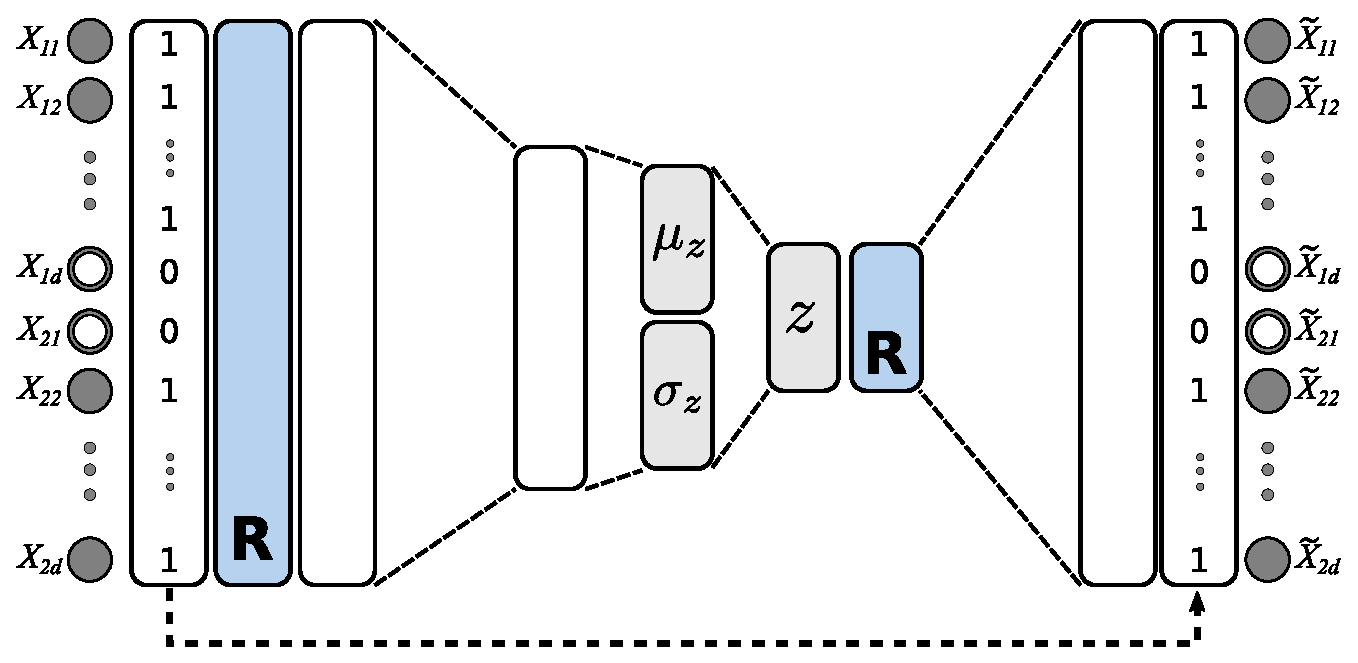
\includegraphics[height=6cm]{img/STEP12_7/VAE_RELEVANCE.eps}
    \caption{Relevance layer}
    \label{fig:my_label}
\end{figure}


\begin{figure}
    \centering
    \subfigure{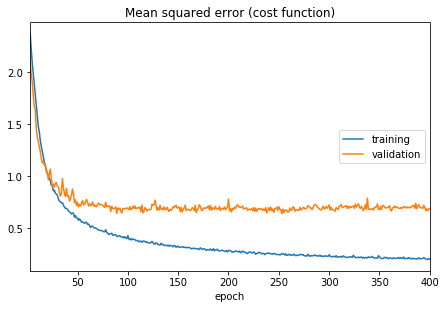
\includegraphics[height=3.3cm]{img/STEP12_7/STEP12_7_pBr2SXR_rm-rs_absarg_training_mse.png} \label{step_12_7_training}}
    \subfigure{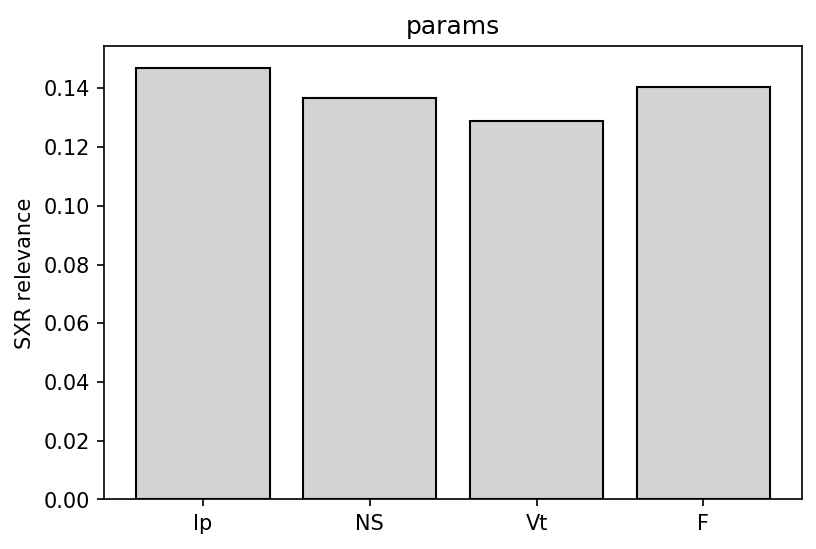
\includegraphics[height=3.3cm]{img/STEP12_7/STEP12_7_params.png} \label{step_12_7_p}}
    \subfigure{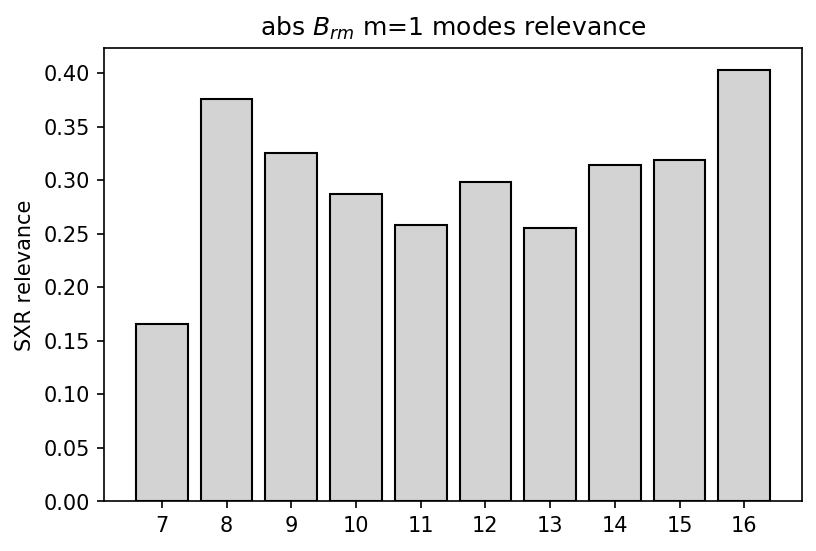
\includegraphics[height=3.3cm]{img/STEP12_7/STEP12_7_abs_Br_rm.png} \label{step_12_7_abs_Brm}}
    \subfigure{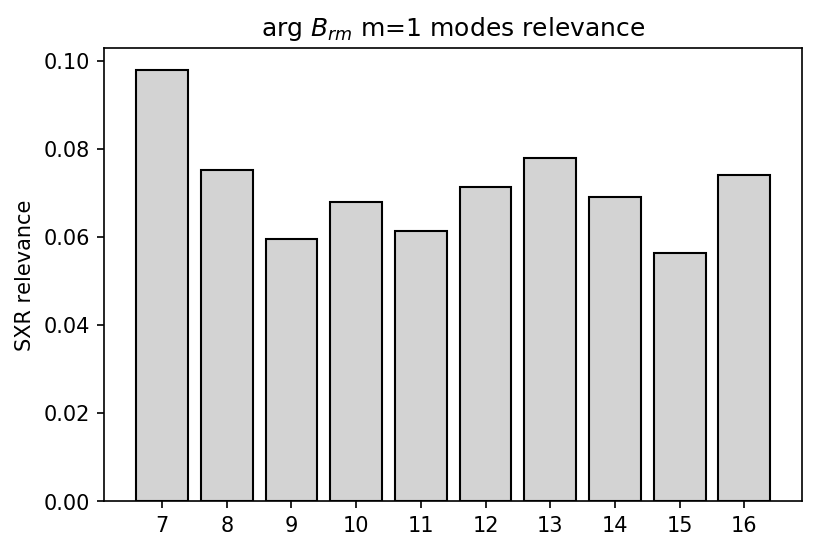
\includegraphics[height=3.3cm]{img/STEP12_7/STEP12_7_arg_Br_rm.png} \label{step_12_7_arg_Brm}}
    \subfigure{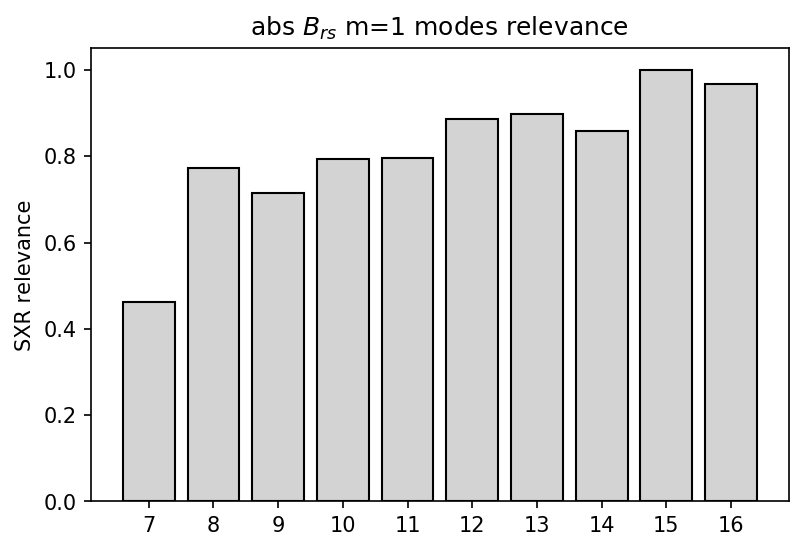
\includegraphics[height=3.3cm]{img/STEP12_7/STEP12_7_abs_Br_rs.png} \label{step_12_7_abs_Brs}}
    \subfigure{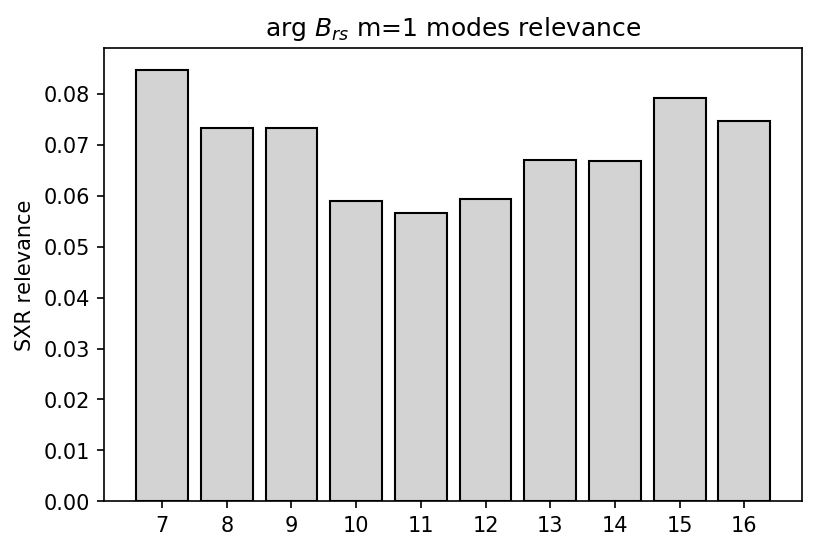
\includegraphics[height=3.3cm]{img/STEP12_7/STEP12_7_arg_Br_rs.png} \label{step_12_7_arg_Brs}}
    \caption{ Training 500 epochs - STEP 12.7 mse, slightly overfitted but validation not diverging }
    \label{fig:step_12_7}
\end{figure}